\documentclass[tikz,border=3pt]{standalone}
\usepackage[T1]{fontenc}
\usepackage{mathptmx}
\usepackage{tikz,pgfplots}
\usetikzlibrary{arrows.meta,positioning,calc,fit,backgrounds,shapes.geometric}
\pgfplotsset{compat=1.18}
\definecolor{forest}{HTML}{346E57}
\definecolor{sage}{HTML}{E8EFEA}
\definecolor{clay}{HTML}{AC653F}
\definecolor{sand}{HTML}{F4EAE2}
\definecolor{ink}{HTML}{252525}
\definecolor{light}{HTML}{F5F5F3}
\definecolor{gridgray}{HTML}{D8DAD6}
\tikzset{box/.style={draw=ink!70,line width=.5pt,rectangle,rounded corners=1pt,fill=white,align=center,font=\fontsize{11}{12}\selectfont,inner sep=6pt}, flow/.style={-{Latex[length=2.4mm]},line width=.7pt,draw=ink!80}, data/.style={flow,densely dashed,draw=forest}, label/.style={font=\fontsize{10}{11}\selectfont,fill=white,inner sep=2pt,align=center}}
\hyphenpenalty=10000\exhyphenpenalty=10000\begin{document}
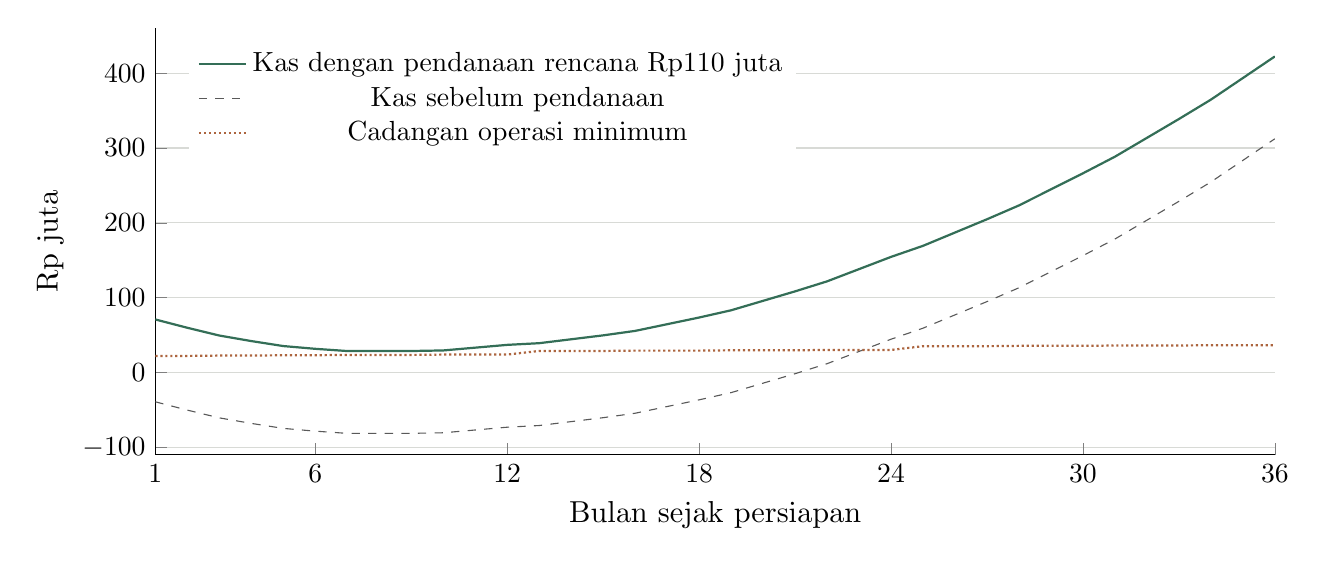
\begin{tikzpicture}\begin{axis}[width=15.8cm,height=7cm,xmin=1,xmax=36,ymin=-110,ymax=460,xtick={1,6,12,18,24,30,36},xlabel={Bulan sejak persiapan},ylabel={Rp juta},axis lines*=left,ymajorgrids=true,grid style={gridgray},legend style={draw=none,at={(.03,.97)},anchor=north west,font=\fontsize{10}{11}\selectfont},tick label style={font=\fontsize{10}{11}\selectfont},label style={font=\fontsize{11}{12}\selectfont}]
\addplot[color=forest,thick]coordinates{(1,70.9000)(2,59.8000)(3,49.4260)(4,42.0320)(5,35.3640)(6,31.6760)(7,28.7140)(8,28.7320)(9,28.7500)(10,29.4940)(11,33.2180)(12,36.9420)(13,39.1920)(14,44.4220)(15,49.6520)(16,55.6080)(17,64.5440)(18,73.4800)(19,83.1420)(20,95.7840)(21,108.4260)(22,121.7940)(23,138.1420)(24,154.4900)(25,169.2640)(26,187.0180)(27,204.7720)(28,223.2520)(29,244.7120)(30,266.1720)(31,288.3580)(32,313.5240)(33,338.6900)(34,364.5820)(35,393.4540)(36,422.3260)};\addlegendentry{Kas dengan pendanaan rencana Rp110 juta}
\addplot[color=black!65,dashed]coordinates{(1,-39.1000)(2,-50.2000)(3,-60.5740)(4,-67.9680)(5,-74.6360)(6,-78.3240)(7,-81.2860)(8,-81.2680)(9,-81.2500)(10,-80.5060)(11,-76.7820)(12,-73.0580)(13,-70.8080)(14,-65.5780)(15,-60.3480)(16,-54.3920)(17,-45.4560)(18,-36.5200)(19,-26.8580)(20,-14.2160)(21,-1.5740)(22,11.7940)(23,28.1420)(24,44.4900)(25,59.2640)(26,77.0180)(27,94.7720)(28,113.2520)(29,134.7120)(30,156.1720)(31,178.3580)(32,203.5240)(33,228.6900)(34,254.5820)(35,283.4540)(36,312.3260)};\addlegendentry{Kas sebelum pendanaan}
\addplot[color=clay,densely dotted,thick]coordinates{(1,22.2000)(2,22.2000)(3,22.6435)(4,22.6435)(5,23.0870)(6,23.0870)(7,23.5305)(8,23.5305)(9,23.5305)(10,23.9740)(11,23.9740)(12,23.9740)(13,28.8175)(14,28.8175)(15,28.8175)(16,29.2610)(17,29.2610)(18,29.2610)(19,29.7045)(20,29.7045)(21,29.7045)(22,30.1480)(23,30.1480)(24,30.1480)(25,35.1915)(26,35.1915)(27,35.1915)(28,35.6350)(29,35.6350)(30,35.6350)(31,36.0785)(32,36.0785)(33,36.0785)(34,36.5220)(35,36.5220)(36,36.5220)};\addlegendentry{Cadangan operasi minimum}
\end{axis}\end{tikzpicture}
\end{document}
